
\documentclass[12pt]{report}
\usepackage{geometry}
\geometry{a4paper}
\usepackage{chicago}
\usepackage{makeidx}
\usepackage{tabularx}
\usepackage{graphicx}
\usepackage{color}
\usepackage{pdfpages}
\usepackage{listings}    
\usepackage{float}
 \usepackage{url}
 
\floatstyle{plain}
\newfloat{program}{thp}{lop}
\floatname{program}{Snippet}



\def\keywords{\vspace{.5em}
{\textbf{Keywords} \linebreak \,\relax%
}}
\def\endkeywords{\par}


\begin{document}
\begin{titlepage}
\begin{center}
\lstset{language=Java}  
% Upper part of the page. The '~' is needed because \\
% only works if a paragraph has started.
\textbf{\LARGE The University of Birmingham}\\[0.35cm]
\textbf{\LARGE School of Computer Science}\\[0.35cm]
\textbf{\LARGE MSc in Advanced Computer Science}\\[2.5cm]

\textsc{\Large Second semester mini-project}\\[2.5cm]

% Title

{ \huge \bfseries Analysing User Interaction On Mobile Devices \\[1cm] }

{\large \textbf{Karthikeya Udupa Kuppar Manjunath}\\[1cm]}

\large{Supervisor: Mirco Musolesi}
% Author and supervisor


\vfill

% Bottom of the page
{\large April 2014}

\end{center}
\end{titlepage}

\begin{abstract}

abstract here.
\linebreak\linebreak\linebreak\linebreak
\begin{center}
\begin{keywords}
keywords here.
\end{keywords}
\end{center}
\end{abstract}


\tableofcontents
\listoffigures
\listoftables
\newpage

\chapter{Introduction}
\noindent
\section{Introduction}
Over the last two decades the world has been revolutionised by technologies beyond what could have been even imagined a century ago. The digital revolution has effected our lives in every possible aspect, mobility is one of the key components of this revolution and has been incorporated in people's live at a very drastic rate [14 -1]. Smart phones and portable devices have become an extension of our persona and have been personalised by us, they reflect our preferences, social choices we make, places we go even the food we prefer to eat. These devices have provided a new meaning to the vision of Mark Wesiser [1] and also a means to achieve more with the growing network of wireless sensors of various kinds in the hands of the people providing realtime information [7]. As we can see in section [x], much work has been done in this direction to make the vision a reality, systems that can provide a groundwork to build ubiquitous systems, algorithms to process the data and make inferences have been developed. This is what we are trying to accomplish in our research as well.

A key component of creating a building block for such a ubiquitous and anticipatory system would be to understand why people perform the actions that they perform at the given time [13] and how it be generalised across the masses which would eventually helps improves their lives without and not be a hindrance, anticipating their actions and adapt itself to their needs [12], Tennehouse [12-43] introduces this concept as proactive computing wherein the system would become so familiar with the user that it would be able to perform action on user's behest.

For us to accomplish this we would need a way in which we can monitor what activities people perform, what are the various contexts which effect these actions and to be able to do this on a large scale. Demographics have been proven to be a very important aspect in extracting features of the user as an individual [12, 4] and also as a collective [6, 3].

This whole process involves a lot of complexities surrounding it, firstly there is an issue of a platform to target, there is also a concern that in achieving such a system we might end up violating user's privacy and interfere in his life all of which among many other are once we address in this research.

\section{Context \& Context-Awareness}
To understand what are the various circumstances under which the user takes a particular action on the device we analyse the \textit{Context} in which the user reacted in the given way. Oxford dictionary defines context as ``the circumstances that form the setting for an event, statement, or idea, and in terms of which it can be fully understood''. Over the years there have been many efforts to define context in terms of computing, [SemI - 30,6,26] all define it in their own way but lack one aspect or the other. In the process that we are doing context would refer to the any information that can define the condition of the user during the interaction between him and the device. This should also cover the relevant state of the device (connectivity, current power level, nearby connected devices among others). [SemI - 8] defines it as``Context is any information that can be used to characterise the situation of an entity. An entity is a person, place, or object that is considered relevant to the interaction between a user and an application, including the user and applications themselves.'' which very clearly defines what our system is trying to accomplish compromising of user, physical, computing and time contexts [SemI -30].

Context Awareness is on the other hand the stepping stone for anticipatory systems. It specifies the ability of the system to firstly know about the state in which it is presently in and eventually adapt itself to the conditions based on its knowledge about the user's preferences. Context-awareness acts as an extension human senses fulfilling its limitation[13] helping in continuously understanding the user's context and improvising itself in its ability to help the user perform his tasks more effectively. Similarly as with all other computing problems, context awareness has moved far ahead from the initial description of context [SemI - 31] with the readily available powerful sensing devices in the hands of masses in the form of mobile phones.


\chapter{Ambient Intelligence \& Anticipatory System}

The field of ambient intelligence and anticipatory systems are closely related to each other, ambient intelligence forms a basis for system which perform anticipatory tasks. Both are a part of what Weiser[x] would have actually thought would come into existence when he said ``The most profound revolutions are not the ones trumpeted by pundits, but those that sneak in when we are not looking''.

The term \textit{Ambient Intelligence} was first introduced in the AmI Challenge in 2001 [E2], wherein it identified AmI at a conceptual level along with components that could be developed to make this a reality. [E3] defines it as an environment wherein the the environment would adapt itself to the needs of the user, there would be a lack of any input devices to take user's feedback instead there would be sensors which would blend in into the environment's day to day items, connect with each other and constantly try to adapt themselves and improve the life of the user. Anticipatory systems as described by [E5] is ``a system containing a predictive model of itself and/or of its environment, which allows it to state at an instant in accord with the model's predictions pertaining to a later instant". Hence, the system itself has to be intelligent enough to make predictions about the future and adapt itself which makes it very similar to ambient intelligence, difference being the ambience of the technology which may or may not be there in the anticipatory system. The current framework and application mentioned further in this report form the ground work for a system which falls into the category of both ambient intelligence and anticipatory system.

\section{Components Of Anticipatory System}
An anticipatory system has multiple components which work together to provide the desired results. As we have seen context forms an essential part of any system that deals with understanding and improving user's day to day tasks and habits. Majority of the information required to do such a task is extracted from the sensors that are available in the devices, however the data as is useless and also usually limited to a single user. We require a larger dataset of multiple individuals that can then be used alongside machine learning algorithms to develop a model and extract meaningful inferences. These inferences can then be used to predict future events and gradually improve itself and its prediction over a period of time in the form of reinforced learning. This process, [E1] categorises into four stages:

\begin{itemize}
\item Sensing of the contextual information of the user.
\item Extraction of feature from data.
\item From the available data make predictions for/about the user.
\item Understand its mistakes and improvise itself to provide more accurate and useful information.
\end{itemize}

Let us further look into each of the above mentioned step in depth.

\subsection{Sensing}
First and foremost step in any anticipatory system is to collect information about its users. The information is usually quasi-continuos sensor reading from the device's various sensors [14] and other similar contextual data that we can gather about the user. The amount and kind of data varies on various factors such as the availability of sensors, portability of the devices and the actual requirement of the system.

With the advent of modern mobile devices we have a plethora of sensors encompassed in a single device which the user is almost certain to carry around and use continuously. This presents an opportunity to for us to extract meaningful information about the user in his natural environment without actually interrupting or obstructing his day to day tasks and without him deviating from his natural flow of work. Almost every smartphone these days has basic sensors such a GPS. accelerometer, light sensors among other and can usually connect to the internet [Diagram 1]. This provides us with a very rich source of contextual information which we can harness for gathering data about the user. This is not just restricted to mobile smartphones but can be extended to various other platforms such as music players (iPod's), tablets, gaming consoles (XBOX, Wii, Playstation), home theatre systems, vehicle GPS navigations and many other components that we interact with almost every day, all of which provide some source of context which we can use.

All the data that was discussed above refers to a person's individual information and is usually referred to as \textit{Personal Sensing}[E7] but with the recent growth in mobile internet networks, people are always connected and so are the devices to both each other and to the web this allows us to not only sense the information but also to provide it onto a central location on the worldwide web. However on a larger scale where we are monitoring a group of individual or a community of people to identify patterns and emerging trends, this is termed as \textit{Crowd-sensing} where in individual's devices collectively provide data to identify phenomena's of collective value to the community [E6]. There are already several real world examples which use community based sensing in areas like environmental monitoring[E6 - 3] and navigation[E6 - 4/5], the only shortcoming of this being unable to interact with the test users personally and take their feedback which can be done with personal sensing.

[Diagram - iOS Context -
- Accelerometer, Gyroscope, Proximity, Ambient Light, Magnetometer, GPS, Bluetooth, Microphone, Fingerprint, Camera, Moisture Sensor

S5 Context - NFC
]

Although sensing, both in terms of personal or community based seems very promising and can provide much in building better systems but are not without their issues and drawbacks. The availability of the data is very much platform dependent, with multiple devices and mobile operating systems deployment is one of the key challenges along with the issues faced on each of the platforms. Additionally as it is with all researches which makes use of user's information privacy of the user and his information is a key concern. We will discuss this further in section \ref{challenges}.

\subsection{Feature Extraction \& Context Association}
The raw sensing data acquired from the sensors whether locally or remotely in the case of crowd-sensing is not of much use to us as raw data itself contains lot of noise, we need to interpret the raw data to extract relevant features based on our requirement. For example we can have the raw data from the accelerometers how do we understand from the accelerometer x,y and z the activity of the user [E8], or maybe the mode of transport which is using at present or if he is just sitting at his house, if the user can be interrupted at a point in time [Intrup Print.]. There are various platforms and statistical tools readily available for each of the data stream. However each data stream might be used to extract different characteristics [E1], for example sound can be used to identify the present surroundings of the user however it can also be used to understand the physiological state of the user as well. So the feature extraction actually depends on what you want to do with the data available.

Another challenge is with crowd-sensing and global distribution pattern using Google Play Store and Apple iTunes store the application usage and in turn the data being gathered can scale at an immense scale. One way to reduce the problem is by removing context information that is of not related or can be ignored, this helps by reducing the load and also by cancelling the negative impact on the results.[12] 

Additionally, there are other co-context's that can be fetched using the available context context information. For example, if our application has some relation to the location of the place the user is in, weather becomes a co-context which can be found with the help of the location context. Similarly, if location itself is not directly available but we have GPS or WiFi information we can calculate the location from it.

\subsection{Anticipations}
Understanding the features and extracting the information from the sensor data provides us with an opportunity to use this information for much more then understanding the present context of the user. By knowing what user's choices are we can make predictions for the future.

From the extracted features various supervised learning models can be constructed which can associate user's activities and the related context. This when applied to the collective data of the community helps us build an effective model which can help us anticipate things for the user both as an individual and for the community.


\subsection{Improvement and Self-Learning}


\section{Components of the present systems and how it related to anticipatory system}

The system in question is a foundation of an anticipatory system, to understand how the system works as an anticipatory systems we need to understand the various components which interact with each other and other components that can be linked with it to make it a complete anticipatory system. The system presently is build for Android mobile platform and supports devices running Android OS.

The primary component of the the system is to gather information for further processing. This task is performed using the context sensing framework, which provides all the context information based on subscriptions. Other then context, user's application usage is also one of the most vital component of the system. This is extracted from the mobile's default API. The framework and the sensing process and strategies are explained in further detail in section [x].

Since the application falls in the category of crowd-sensing, the data is sent to a central data store on the web from the various devices of individuals. The application makes sure that the data is sent to the server in a power and money efficient manner (See section [y]). The server is responsible for storing the information securely and also acts as an authentication server. Essential features are filtered and context is associate with each other and the user. Further also tries to understand the extracted information and provide end points for the application to get prediction data and analytics information (See section [z]).


\chapter{Android Context Sensing Framework}
\label{ContextSensingFramework}
Context is a very primal component in all of the anticipatory systems. As one can conclude from [Figure 1], the contextual information that can be gathered using modern smartphones is a lot, more and more sensors are being added onto the devices. However, there are various mobile platforms and each consisting of its own development environment, tools and deployment stores making it very difficult to develop a framework which can function on multiple platforms. For the purpose of this project selected the Android development environment for various reasons.  The platform this provides a much more flexible and open framework to extract contextual information. It also the most widely used mobile operating system and consists of devices of all price ranges hence providing a much more diverse target audience.

Although there have been many contextual frameworks in the past some of which are for Android as well; providing an relatively easy methodology to extract meaningful information \cite{novakextensible2013, rachuri2010emotionsense}, however the present requirement of the project is much simpler and there are some components that the frameworks presently do not monitor, for example, \cite{novakextensible2013} does not monitor network, WiFi access points, \cite{rachuri2010emotionsense} does not monitor user's schedule and phone profile. Also a framework at this point would provide more flexibility and access to the more recent API's which older frameworks do not cover. Although The context sensing framework designed for the purpose of this project but it is designed in a way to interface and connect to any application for monitoring purpose.

\section{Contextual Information types}
\label{contextType}
There are various sensors that are available for the purpose of monitoring in the modern mobile devices and supported by the Android SDK. The following are the contextual information which were considered to be supported and available for subscription in the first version of the framework.

\begin{itemize}
\item Location (GPS or Network)
\item Battery/Power Source Information
\item Network Connectivity Status
\item Network Signals (Cell Tower Connectivity)
\item WiFi Access Points and Connectivity Status
\item User Events
\item Bluetooth Status and Nearby Devices
\item Telephony Events
\item Screen Activity Context
\item User Phone Profile (Screen Brightness, Volume Settings \& Vibration)
\end{itemize}

We will further discuss a few of the the above mentioned context's in details and how a scanning methodology was customised for it be both effective and efficient.
 
\section{Framework's Working Architecture}

In order to understand how the framework would actually function once integrated we divide the system's architecture into two components, first is the external end points of the framework which any application can interact with the second component is the actual internal component which handles subscriptions, monitoring, polling and content delivery.

\subsection{End-points and External Handling}
\label{ExternalHandling}

As we described earlier the purpose of creating a new framework is to make sure information is provided in the simplest possible way and should be extensible. Also the framework has to be plug and play, there should be very minimal code that would have to be written on order to integrate it with an existing application and to perform what is required. The functionality of any existing application should not turn away from its original goal to focus on the integration of the framework and procuring data from it. The framework should just be a component integrated into the application providing a stream of required information and which can be controlled by the application.

The framework's architecture can be described as a subscription based model, wherein each of the components can be subscribed externally by the connecting application. In addition to that each subscription can be provided with additional parameters in order to tailor the subscription based on the needs of the application.

To begin monitoring any particular context one just has to call the \textit{monitorContext} method from \textit{ContextManager} object. The call then initiates a monitoring service for the context based the parameters that is being passed with it.

\begin{program}
  \begin{verbatim}

public void monitorContext (
            ContextManagerServices mService,
            long minimumUpdateTime,
            long pollingTime,
            ArrayList<Integer> flags
    );
\end{verbatim}
\label{monitorContextCall}
\caption{Function definition of the monitor context.}
\end{program}

As we can see in the function call, there are several parameters, let us look into them for more detailed understanding of the function's actual functioning.

\begin{itemize}
\item \textbf{\textit{ContextManagerServices} Parameter - } \textit{ContextManagerServices} is an enumeration defining various types of contexts that can be monitored by the framework [see Appendix 1], this specifies which context the application wants to monitor using the framework.

\item \textbf{\textit{minimumUpdateTime} Parameter - } This specifies the minimum time the application should wait before sending a forced broadcast about the context regardless if there is any change in the context or not. This is useful for application which want information about context at regular intervals regardless of the magnitude of the change.

\item \textbf{\textit{pollingTime} Parameter - } This parameter specifies the time interval after which the framework should poll the sensors or the operating system for information about the context. This is specifically for information which do not have system provided callbacks (Broadcast/Intent architecture) and require polling or in cases where power consumption for constant monitoring is too steep and is not feasible (e.g. GPS based location monitoring).

\item \textbf{\textit{flags} Parameter - } This is an extensible parameter which is essentially an array of flags which can be passed to the framework. This also provides a backward compatible way to extend the framework without changing the original function call. An example for the use of this parameter is for passing information about the source to use for location tracking to use while performing the polling task.

\end{itemize}

With the help of this one call, one could start monitoring any contextual information that is made available in the present version of the framework. In case of missing timing information in the call, the framework uses a different constant value for monitoring tasks.

[Figure 2 - Broadcast Intent Receiver Arch.]

To notify the application about contextual information the Android platform provides a very effective methodology to transfer information between the framework with the help of \textit{LoalBroadcastManager} which sends a message called \textit{Broadcast} to all the \textit{BroadcastReceiver}. The working of the methodology is very simple yet very effective. As [Figure 2] explains we can ask for an object to register itself to the \textit{LocalBroadcastManager} to be notified in case it receives a broadcast with a particular name or tag which is referred to as \textit{action} in Android.

The framework uses the same flag for all the notifications with more detailed information inside the \textit{Bundle}.

[Figure 3 - Framework Architecture]

The application would have to register just once to the\textit{LocalBroadcastManager} for any and all context's it is monitoring. When the framework has an update it would send a broadcast, which would have the following components:
\begin{itemize}
\item \textbf{Action - } All broadcasts from the application are associated with one action string `\textit{CONTEXT\_CHANGE\_NOTIFY}' regardless what type of context it is.
\item \textbf{Additional Information - } Other then the action, broadcast can also contain addtional information in the form of a key/value pairs. The framework sends various other values for each broadcast.
    \begin{itemize}
    \item \textit{CONTEXT\_TYPE - }The type of context the broadcast contains. [See appendix 2 for detailed list.]
    \item \textit{Context Information Flag - }This flag is named after the context type that is passed, hence varies depending on the content it contains, the value is a JSON (\textit{JavaScript Object Notation}) formatted string containing information passed by the framework.
    \end{itemize}
\end{itemize}

Finally, the application should be able to stop monitoring a context as easily as it begin monitoring the context. The context can be stopped from being monitored and hence the application would receive no further updates by simply calling

\begin{program}
  \begin{verbatim}

public void stopMonitoringContext(
            ContextManagerServices mService
        );
\end{verbatim}
\label{monitorContextStopCall}
\caption{Function definition to stop monitor context.}
\end{program}

\subsection{Internal Working}
The internal working of the framework relies on multiple components of the framework interacting with each other. As described in section \ref{ExternalHandling}, \textit{ContextManager} is the external interface with which any application trying to use the framework would interact with. The class is also responsible for delivering broadcast at \textit{minimumUpdateTime} intervals. However, the framework works on a set of classes which ensure that latest information is always available and done effectively.

A singleton class, \textit{ContextMonitor} is primarily responsible for performing monitoring at the given time intervals and updating the context values for the \textit{ContextManager} to use. There are two kinds of contexts that we have to deal with.

\begin{itemize}
\item \textbf{Polling Tasks - } Certain contexts need to be accessed using Android system API calls at the required time intervals, for this the we use a timer task in \textit{ContextMonitor} is initialised to do the polling task for it. In case there is an update in the information a broadcast is sent to all listeners about it.

\item \textbf{Monitoring Tasks - } Some of the available contexts have a broadcast and intent model provided by the system itself, so in this case, a broadcast receiver object for that particular action is created in the singleton to receive information and update its variables accordingly and in case of a relevant change a broadcast is sent to the receivers.

There are several advantages of using the development model, primarily this provides a single point of access to all the information that is required by the framework which in itself is very beneficial in scaling the framework further. Additionally, a single instance of the monitoring task ensures there are no multiple tasks being run by the framework in case the application using the framework starts to monitor same context at multiple places. Although, this might look very minimal but for polling tasks like location information and bluetooth scanning this is very effective in terms of resources spent.

\end{itemize}


\section{Understanding individual context monitoring}
Each of the context's being monitored by framework have their own unique methodology in which they work. The uniqueness helps them to perform monitoring in a very effective and power efficient way. Let us look in details a two of the important context's working.

\subsection{Location}
Location, one of the most important contextual information that can be extracted. With modern devices which people carry everywhere it has become all the more important. The major concern with location is the power consumption factor when using GPS [E14], so constant monitoring of GPS is never recommended on mobile devices. Also, time it requires to switch on the GPS sensor and get a triangulation from the satellites can also be a concerning factor sometimes. Modern devices provide network based location services which require both network connectivity and internet to provide location. This process is battery efficient but accuracy is usually questionable. 

The framework provides the application option to opt for either of the technique in addition to the ability to specify the polling interval.

[Figure 4 - Location Working]

Android operating system itself stores the last known position [E16] which is updated when any of the application triggers the location manager. So at the given polling interval the device first looks for location by using the \textit{getLastKnownLocation} method. Then the system analsyes if the location that is been provided by the system is a better location then the one it already has and if it meets the criteria (freshness of the location), if the criteria is met this location is stored and broadcasted. If not, the system would trigger the specified location provider (GPS or Network) to provide it with a new location, the fetched location is then broadcasted and stored.

\subsection{Network Information}
Mobile phones are usually connected to networks, when the user moves the connection to the network also changes. The systems decides which signal providing tower to connect to out of the ones that are available. This information can be very useful in terms of context. For example with this information one can map the network density and signal strength of the area. There are several components that constitute of network information and there is not a single method to monitor this.

[Figure 5 - Network Working]

\begin{itemize}
\item \textbf{Signal Strength - } Signal Strength constantly changes and can be monitored by a system provided broadcast receiver. However the frequency of the change is very high, hence broadcast is done only when there is a significant change.

\item \textbf{Cell Towers Nearby - } Although the device usually connects to a single cell tower but there are various other towers which broadcast their presence and the device picks it up along with other information such as their signal strength. This information is also provided through a broadcast receiver by the system.

\item \textbf{Data Connectivity - } The networks may or may not be providing data connectivity to the device or the user might have turned off the data connectivity. This information needs to be polled constantly as the broadcasts are not reliable and do not provide internet connectivity information. The framework frequently checks for updates about connectivity information and notifies if there is any change.

\end{itemize}

\section{Shortcomings \& Possible Improvements}
\label{contextShortcomings}
The framework provides a foundation for a much more extensible and useful framework for android. There are several areas which should be considered in the future versions and will improve it further.

Firstly, the framework can be made more robust, currently it has been designed for devices running Android version 4.0 and 4.4, backward compatibility would certainly make the framework useable on a wide range of devices. 

Although android is at present one of the most popular operating system in the mobile arena, there are a considerable number of the mobile users who use other popular operating systems like iOS and Windows platform, an extension of the sensing framework with similar functionality (within the bounds of the operating system) on other platforms would be certainly helpful in conducting studies with a broader group of audience then just people using android.

Additional context's like accelerometer and application monitoring (currently implemented in an external app using the framework) are presently missing in the framework and would be a valuable addition to it.

The sensor information gathering technique is primal in nature and lacks adaptive qualities like in EmotionSense [E10], which allows the sensing to be done adaptively instead on a fixed interval. For example movement of the user should be tracked based on the movement he has done during the last interval, if the location change between two interval is considerable less or none, the next sensing should take place an increased interval or if the change is considerable the sensing time interval should be reduced. Additionally, it should take into consideration the battery usage of the sensor and the current state of the device, i.e. sensing intervals should adapt itself based on the battery life of the device.

Given enough time the framework can be expanded into a much more robust, functionally rich and highly customisable component which can be used in various kinds of studies and real world application. 

\chapter{User Smartphone Usage Data Collection Application}

The most essential goal of this project is to devise a technique to gather information about how a real world user interacts with his mobile device on a day to day basis in his natural and unmoderated environment. The context sensing framework provides a very robust foundation using which we can gather information about the context in which the user is using the mobile device. But at present the framework does not consist of any possible way to monitor and gather information about mobile phone interaction of the user both in terms of web and application usage.

\textit{WebSense} is an application for the Android platform developed for the very purpose of collection of user application usage data collection along with the related contextual information. The application is integrated with the context sensing framework described in chapter \ref{ContextSensingFramework} which it uses to extract contextual information of the user.

There were two aspects of the application which were taken into consideration while designing the architecture of the application. First was the actual development of the monitoring functionality to provide an efficient way that was to be used to monitor how the user interacts with the device in a ubiquitous way and eventually send it to a central data repository on the web for collective analysis. Second aspect was the utility value it provides to the user which is essential for crowd-sensing application as apps in the crowd-sensing domain should be lucrative enough for people to install even if they are not interested in the research value of the application (see section \ref{PlatformDeployment} for deployment challenges). In the following sections we look into each of the aspects and the various components which collectively provide a skeletal over which the application functions.

\section{Application Usage Demographics Collection}

Android is a very open platform in terms of providing access to data sources when we compare it with the other most popular operating system for mobile platforms such as Apple's iOS \cite{AppleiOSPolicy}. This allows us to develop application which can monitor user interaction in detail.

The most essential criteria of any monitoring application is to maintain a near 100\% uptime, which means that the app should always be running in the background and performing the necessary operations. Implementing a front end interface provides user an option to terminate the process very easily by accident or intent hence denying the change of gather information. However a background service on the other hand is more complicated to be terminated and also ensures that no hinderance is caused to the user in performing his day to day mobile phone usage. Hence the architecture of the app consists of several of background services each with their own set of responsibilities. This, along with a design to ensure that the monitoring service is switched on in case of device restart, accidental termination by the operating system or in case of an internal malfunction causing the termination of the application provides the system to operate at a near 100\% uptime (see chapter \ref{PeformanceEval} for detailed evaluation).

[Figure = Application Monitoring Architecture]

Let us look into the various background services along with their role in the overall architecture of the system.
 
\subsection{Application Usage Monitor}

The primal responsibility of the app is to monitor the user's application usage continuously and with certain level of dependability. This task is performed by the service \textit{AppUsageMonitor}. The service is a self-reviving service so in case it is terminated either by the operating system or due to a malfunction it revives itself within a matter of seconds, ensuring an almost 100\% uptime.

Since Android does not provide a broadcast or any sort of delegation methodology to know when the application is switched, the only possible approach to do this at present is a quasi-continuous monitoring of the device's application stack. An interval of 4-second was chosen between each scan since research has indicated that user's attention span switches between the device and the environment somewhere within this duration \ref{oulasvirta2005interaction}, hence we can assume that the user would switch applications as well at around the same frequency. Android provides access to the the list of currently active processes through the \textit{ActivityManager} class. The class not only provides information about the running tasks but also provides a mechanism to access the order of the application's screen presence. With this information we can identify which application is currently running and being interacted with on the device by the user.

Android also equips its developers with intents which one can listen to for detecting user's action of turning the device's screen on and off. This allows us to stop monitoring user's activity tasks when the phone is turned off hence saving crucial resources.

The application uses SQLite database\footnote{ self-contained, transactional SQL database engine - https://sqlite.org/} to store the monitoring information. This includes package name of the application, start time, end time (Both in UTC timestamp format), duration of the run, location it was used at (subscribes to the framework, listens and stores location information constantly) along with the day of the hour the application was used at. Additionally, a flag marking the synchronisation state of the record is also maintained. 

Whenever an application switch is performed the data is written into the database hence minimising the chances of data lose incase of a malfunction or termination. The information is also saved in the scenario when location update is received while an application is running, hence splitting a continuous session of the application based on the location. This is particularly useful in case of navigational applications as the user would keep it open over an extended period of time while his location changes constantly.

If the application is detected to be the default browser of the device, the app also gathers information about the page user is presently viewing. Although, there is no direct way to perform this, android provides an API to access browser history\footnote{Browser Data Provider - http://developer.android.com/reference/android/provider/Browser.html}, the most recent record in history would be the page the user is viewing currently. Whenever user changes the URL a new record is created and hence the time spent on a particular URL is also recorded.

\subsection{Contextual Information Monitoring}
\textit{ContextBackgroundMonitor} class is also a background service which is responsible for registering and monitoring the contextual information. Presently it monitors all the contextual data provided made available by the framework (see section \ref{contextType}). It is responsible is to make sure that as soon as the service is initiated it subscribes to all the available contextual information provider and whenever there is any new information made available by the framework it saves it in the database. Since we require information about location for mapping the information geographically and also have to provide user with information in relation to his location, all the context information is stored along with the latest location information attached to it.

The class is initiated as soon as the monitoring begins and when the class is destroyed it releases all the receivers and initiates the stop procedure in the framework (see section \ref{ExternalHandling}) hence stopping monitoring process altogether.

\subsection{Web Synchronisation Service}
The context sensing and the application usage monitoring generates a considerable amount content in terms of memory. This can directly used for the purposes of local mining (see section \ref{AppUsageInfo}) but this being a crowd-sensing application, we need the information at a central location to further analyse information of the user-base as a collective. For this purpose, the information that is in the local datastore has to be constantly sent to the remote server on the web.

The class \textit{SyncManager} performs all of the synchronisation of the device with the web by uploading the information in the most efficient way possible. After a certain interval of time the class triggers a method to check for a possibility for a need of uploading of the information. Records which have not been synced in the database is the first criteria the method checks for. To avoid repetitive reads to count un-synced records the monitoring services automatically increments the count whenever a new record is added and stores it on a preference file, this file is read by the synchronisation process. If the criteria for data upload is met the information is uploaded in chunks of fixed number of records in the form of a JSON string and once the data is successfully uploaded the records that were sent are marked as synced. The synchronising process uses the end points provided by the web application and sends the data after compressing it using GZIP \footnote{GZIP File format specification -http://tools.ietf.org/html/rfc1952}. The records are sent with an authentication key to both validate and associate the records, this key is obtained during the login process (see section \ref{LoginInterface} and \ref{StoringInfo}).

[Sync process algorithm - Criteria]

The service is also responsible for periodically clearing old data which has been synced already and are beyond the time-period which is relevant to the application (30 days in this case).

\section{User interface \& Providing utility value to the user}

The monitoring and reporting aspect of the project could have been done without actually a front end with everything entirely handled by background services but the primary test subjects of this application are not a selective group of people, like any crowd-sensing application the future research based on this application tends to make this available to as many users as possible, not only the people who are interested in the research aspect but common public with Android devices. As we will see later on in chapter \ref{challenges} one of main issue when dealing with crowd-sensing application is that it is bottle-necked by the fact that the entire research, application's widespread usage and the amount of data gathered depends solely on the decision of the user to install and keep the application on his phone. So to ensure widespread participation and retention of the application we need to provide the user utility value through the frond end of the application, so regardless if the user is concerned with the study or not he would still have a reason to install the application.

The user interface of the application which runs atop the data gathering services provides 
information and feedback to the user and also helps in gathering certain user's personal information.

\subsection{Login/Registration interface}
\label{LoginInterface}

The login/registration interface is the initial screen of the application where in the user provides the below mentioned information if he is registering or just logs into the application if he has already registered.

\begin{itemize}
\item Email Address - Allows us to have a medium to contact the user in the future.
\item Password - For authentication purposes in case the user logs out or wants to login on another device.
\item Gender - Can be used as an metric to perform future studies.
\item Employment Status - Additional parameter which can be used in future studies.
\item Consent to allow monitoring - Along with a link to the End user's license agreement.
\end{itemize}

The application allows multiple sessions using the same credentials on multiple devices. An option to log out of the application is also provided inside the application, in case the user wants to do something privately or wants to stop monitoring completely.

\subsection{Application usage information}
\label{AppUsageInfo}

Application usage of the user is being constantly monitored by the application in the background, this interface provides a view by accumulating the total usage over a certain period of time. The interface provides information about the total usage in a very visual way allowing users to compare the various application. An option to filter the information to a particular duration (day, week and month) is also available.

\subsection{Application and web usage trends}

This provides similar as the previous screen but instead of providing information for user's application usage, it provides aggregated information about the trends throughout the user-base of the application. It shows the trends of application usage based on the data accumulated over the period of time on the web server over a period of time. The web API has an end point which provides the information for the required duration of time (day, week or month).

The application's information is also provided along side, hence icon and the name of the application is shown along with an option to install the application if it is not already installed. This acts as an recommendation system for the user to try new application based on popularity.

Along with the application usage trends the app also shows information about the web usage trends, showing information along with some content and images from the websites popular among the masses in the given duration.


\subsection{Localised web and app usage trends}

The information about the app and web is can also be restricted to the present geographical area. The app has the capability to present the user information about what is popular in the user's current area. This can be very helpful for example, if the user is opens the application at a train station the app would provide information about the apps and websites people use there, which are most likely to be the ones providing information about the the timings of the train.

The geographical radius is decided on the server the location is provided by the context sensing framework which then is passed along with the web request. The process of handling this request is discussed further in detail in section \ref{ExtractInfo}.

\section{Web API and Feature Extraction}

As we have seen the application provides a robust yet lucrative way for the users to provide their application usage information, however in order to achieve this at a larger scale and not just for a single user we need a web server to handle storing of information, extract features and finally process it to provide meaningful information for the application to display and even perform predictive tasks at a later stage. For this purpose a web application was build and deployed on the internet. The application is build using Node.js \footnote{Even-driven JavaScript backend - http://nodejs.org/} which provides a very reliable framework to build high performance web API's,  dealing with an increasing number of web requests \ref{tilkov2010node} which is bound to scale over time. The datastore for the application is a MongoDB\footnote{Non-relational, Document based database - https://www.mongodb.org/} database which provides various functionalities to process and extract information efficiently. It also provides lot of features to improve handling of high request rates and take care of the needs for scalable systems.

The web app is essentially a collections of RESTful API end points with JSON data format to store, process and provide information, all of whom incorporate GZIP compression in their requests and responses to decrease bandwidth being used. It also constitutes of a analytics dashboard which showcases various metrics from the server. Let us briefly go through the available API endpoints and their internal working.

\subsection{Storing Information}
\label{StoringInfo}

The application stores various types of information. The first possible request an app can make is to register or authenticate the user. The information about the user is stored in the \textit{user} collection. The user document is designed to handle multiple devices and multiple sessions running simultaneously. The document model also stores other information that is sent by the app when the user registered which can be used as a research parameter for future studies.

When authenticated the service checks for the user record along with the device information and either creating or updating the device information that is provided with the login information and returning a unique authentication key which can be used for all further requests.

Storing of web and app usage information is more complex, when the service is called the first thing the server checks is if it is a valid service in terms of the authentication key that is being supplied. If it is, then it starts processing the information that is provided. The user is almost instantly provided a OK status message while the processing is going on.



[Figure app processing information]


It collects all the package names that were sent in the request and checks the existing collection of application information for their records, the ones which are new are then sent to a different service call which asynchronously checks each of the package name and fetches information about the application from the app store by scrapping the web page for information. The location information is also corrected and stored in the required format to perform geospatial queries later on.

The process for storing context information is also identical, except there is not much processing at present and once the information is cleaned and converted into required format it is directly pushed into the \textit{context} collection.

\subsection{Extracting meaningful information and patterns}
\label{ExtractInfo}

The web app is also responsible to identify and provide patterns identified from the stored information to the application on the device about application and web usage. The information is extracted from the database using the MapReduce technique which MongoDb supports. The details of the technique are explained in the Figure [x].

The process for extraction of information usually involves aggregating the app usage for each package, however,this can also accommodate filtering based on parameters such as like duration and location information. Location filtering uses the geospatial functions that is provided by mongoDB to reduce the records to a particular area only. The radius along with things such as packages to ignore can all be configured in the config file for the server allowing dynamic changes to the server. The diagram above shows in depth the working of the functionality.

\section{Possible Improvements}

The application and the framework were both developed over a period of 1.5 months. The purpose of this project was to lay an initial foundation for a robust data gathering application along with a framework which would be re-useable component for context extraction both of which can be re-shaped and used for studies beyond the scope of the present project. This being said, there are various improvements that can be done in the existing application and its web counterpart.

\subsection{Android App - Shortcomings and possible improvements}

The android application has a few shortcomings in this first release which can be improved over the period of time. 

\begin{itemize}

\item Firstly, any improvements that were mentioned in relation to the framework (see section \ref{contextShortcomings}) would effect the overall performance of the app, both in terms of resource consumption and the amount of data that can be gathered using the application.

\item The application at present fails in monitoring web usage if they not performed on the default browser which is accessible by the Browser data provider (\textit{Chrome} on Android 4.0 and above) in the Android SDK. This can effect the overall demographics of the web usage data being collected as interest of the users using other applications to browse internet would not be registered by the application.

\item The application also fails at monitoring tasks which can perform their functionality in the background while user is either using some other application or has switched off the device's screen for example applications such as music players and radios can play audio for the user while running in the background without having the front-end open.

\item The application presently provides analytics and trends information which is very generic which can be customised and converted to a personalised recommendation system among various other possible improvements that can be done to provide more value to the user as an utility application (see section \ref{RecommendationSystem}).
\end{itemize}

\subsection{Web Component - Shortcomings and possible improvements}

The web component can be improved considerably by adding more features and also by improving overall performance and scalability of the system.

\begin{itemize}

\item The web component at present does not deal much with the context information, it just uses app usage and location information to provide the various results, future features can make use of all the available information both for research purposes and also for implementing in the application. 

\item The web component's security can be improved by using \textit{Bcrypt}\footnote{Bcrypt: Bowlfish file encryption - http://bcrypt.sourceforge.net/} to store and encrypt private information. Additionally, more precautions can be taken by disassociating the contextual data from the user (see section \ref{UserPrivacy}).

\item The database connection at present picks a connection from the connection pool of the driver, which is a reusable pool of already active connection helping in reducing frequency of opening and closing of connections \cite{MongoLab2013}. There are several things that can be done to improve the speed network transactions.
    \begin{itemize}
        \item Sharding\footnote{MongoDB Sharding - http://docs.mongodb.org/manual/sharding/} maybe applied and to the MongoDB instance to improve the performance of the application and handle increase in the data needs.
        \item At present whenever there is an API call the web service triggers the MongoDB driver along with its customised query which reads from the database process it and returns it back to the service to be delivered further to the device. Considering the number of records being created by the devices, once this application has become widespread this process would start taking more and more time to process the request. A caching layer which would store the information in memory instead of reading raw information from the database and processing it again can improve the performance of the queries. Technologies which are meant to handle rapidly changing content in the memory such as Redis\footnote{Redis: An Open source key-value datastore - http://redis.io/} can be used for this purpose in the future.
        
       \item Use of MapReduce technique to perform various complex functions in the application benefits the overall performance, but at present each time the service is called the MapReduce process is performed. This can be avoided by using incremental MapReduce\footnote{MongoDB: Incremental MapReduce - http://docs.mongodb.org/manual/tutorial/perform-incremental-map-reduce/} which automatically reduces the information when new information is added incrementally hence reducing the load on the server by a considerable amount. Future implementations can also look into a Hadoop based MapReduce implementation on the existing MongoDB instance as it has shown promising results \cite{dede2013performance}.
    \end{itemize}

\end{itemize}



\chapter{How can the information collected be used}

The primary purpose of this stage of the experiment is to design an effective method to gather information from the user on a large scale along with an effective delivery method. The information being gathered is presently stored and and basic feature extraction techniques are being used to provide analytics and trends within the community and in a certain geographical area. However considering the diversity and richness of the data that is and will be available as a result of this application can provide useful input to serval interesting areas of research and help develop various practical applications.

Let us look at a few possible novel approaches to use the information that has been gathered in the near future.

\section{Intuitive Application Launcher}

A very simple application on the lines of the FALCON system \cite{yan2012fast} which we are already working on would be to build an intuitive launcher for Android devices based on the predictions that would be derived from the gathered information. However, rather then actually launching the application we can provide a much more simplified approach by not pushing the user to make a choice and saving considerable amount of resources.

[F10]

Mobile devices usually turn their screens off if there is no activity from the user. Whenever user has to use the device the screen has to switched on and the lock has to be opened. In the event of the screen being switched on, the application which would be integrated with the device's lock screen would present the user with options to launch certain applications. The list of application for the user to choose from would be modified based on time and location. This kind of predictive computing can be very helpful for the user and can prove to make the user's smartphone usage more efficient.

We already have contextual information about the user along with his application usage pattern which we can associate to extract a possible list of application he might want to use. An effective development method with the processing divided between the device and the server would be required to make sure the list can be provided without internet connectivity.

Additionally, the application can learn and improvise itself based on the choices the user makes on the launch screen, i.e. whether or not user selects an application from the list that was provided hence making the application better at predicting application selection over time.

\section{Recommendation System}
\label{RecommendationSystem}

the present version of the application provides recommendation in the form of \textit{What's Trending} using the information that is available about the user's app usage and the location context. The recommendations however are very generic in nature, i.e. recommendations on the basis of the user-base or geographical area. There can be several improvements to the existing feature. The system could recommend users what is trending based on their mobile usage pattern, for example if a person uses a certain application for ordering food frequently and there is another application which is popular in the geographical region the application can make a suggestion to him to try out the other application. The prediction can also be influenced by other information that we have collected like gender and user's employment type.

A similar feature can also be developed for the web usage. A recommended reading list can be compiled based on the user's reading habits and the present trends. To achieve this in practicality would require natural language processing to analyse the content of the webpages to understand the relevance of the link. The application would have to understand the user's web usage pattern and derive a web profile for the user and improving it over a period of time based on user's choices and web usage. The content which is recommended is already popular among people the possibility of a favourable recommendation is more likely. This would be similar to the idea presented in \cite{BalabanovicAWP1997} but would be for mobile devices. Which would help the system to learn and adapt faster.


\section{Content \& Application Pre-Caching}

Information gathered about content being accessed on the web or application being launched alongside the location context provides us an insight about what is popular in a particular geographical region. This as discussed earlier can be personalised to provide what user tends to view or use at a particular location frequently. Application can be launched and kept running in the background as to reduce the wait time for the user when the application is launched and possibly loading itself into the memory or maybe loading content from the web.

[Web caching Interface Diagram]

In relation to the web, this information can be used in a very different scenario. With the knowledge about localised trends on the web an interface can be created which can be made accessible externally to provide possible websites people might use at a particular location. This information can then be linked with the local cellular network or WiFi access points and the content can be cached on the network itself provided improved loading time for the users of the network hence improving the overall user experience. This can be further improvised further by anticipating and then caching possible future navigation from the current website reducing the loading time of requests even further beyond what is achievable using the trends information \cite{cheluvaraju2011anticipatory}.

\chapter{Performance Evaluation}
\label{PeformanceEval}

\chapter{Challenges \& Concerns}
\label{challenges}

As with any research, there are several challenging aspects and concerns that are to be considered both in terms of the present scope of the application/framework and in terms of the future prospects where the research can be used. Let us briefly look into some of the consequential challenges that are to be concerned.

\section{Platform Restrictions \& Deployment}
\label{PlatformDeployment}
The framework and the application in this report were both developed to be used on Android operating system, this restricts the user who can participate in the study to only one's with a smartphone which runs Android and users with other devices cannot contribute to the study in any way. 

This not only can cause an overall decrease in the number of participants, it can also effect the demographics and the data collected as there can indeed be a variation in smartphone usage based on the operating system. Even though \cite{gartnerMobileSurvey2013} shows that Android holds a majority among the masses in mobile marketshare, there are still a considerable marketshare using other operating systems and also the demographics of operating system usage can very widely across geographies. This presents a very serious concern and also a possible direction to look into in the future research as it is being faced by other researchers involved in similar crowd-sensing applications \cite{balan2011real}. 

However, Android is a very flexible platform which lets us build applications which can access such a wide array of information lot of what is currently not possible on other operating systems such as iOS. iOS, for example is governed by a sandbox policy \cite{AppleiOSPolicy} which does not allow to application to access information beyond its assigned limit (such as extracting information about the running applications).

Also, being a crowd-sourcing application, it is to be installed from a application store for android which presents another problem. This puts the decision of participation in the study solely on the fact that the user recognises the application on the store, installs and retains it on his device. The participation rate would vary depending on the application's popularity and would take some time to provide a considerable dataset which is explained further in \cite{xiao2013lowering}, it also recommends on how to remove installation of the application from the critical path but is presently not possible on Android for the type of information we require.

\section{Resource Utilisation}

The purpose of the application is to monitor the how the user interacts with the smartphone and to observe the various contexts and sensors, which means that it has to quasi-continuously execute series of scans and poll sensors/API's in order to extract the required information. The extracted information has to be stored on the disk and also has to be sent to the web server frequently for analysis using the internet connection of the device. All of these processes require a considerable amount of processing power, battery power and internet bandwidth (which in-turn means the user may incur some monitory expense), hence making this a very critical aspect of the application which would have to be optimised.

For the application to be able to gather realistic information from the user it requires to be able to do it in an ubiquitous way, which would not be possible if the application is consuming too much of resources hence causing reduction in the average battery cycle of the smartphone or reducing the data bandwidth available to other apps hence making the connectivity a bottleneck for other application and causing the user experience of the applications to deteriorate. 

Making the application perform all the required tasks while being efficient enough to have a very minimal footprint on the device was one of the key challenges of the project. Various steps were taken during development to make sure that the resource utilisation is kept to a minimum (see chapter \ref{PeformanceEval} for detailed evaluation). For example, the application has an optimised synchronisation process, it prefers synchronisation of records on a WiFi connection rather then a cellular data connection, however if a threshold is reached in the collected information it tries to synchronise on cellular data network to reduce changes of data loss. The polling tasks of the framework are programmed to be functioned at fixed intervals which are specific to tasks and has a direct correlation with the type of information it provides, power consumption and required level of freshness of the information.The overall polling of context is done by the framework at certain fixed intervals each reflecting on the power consumption and the requirement for freshness of the data.

The resource utilisation can further be improved by developing the framework to perform adaptive sensing instead of scanning at fixed intervals. We can also do some pre-processing on the data (e.g. remove non required elements) hence reducing the overall bandwidth usage of the application. Deriving a relation between sensing rate and the power level of the device can help improve the battery life of the device. Sources of information which consume lesser power should be given preference for example using network instead of GPS for location detection is proven to save resources with an acceptable location accuracy \cite{zhuang2010improving}.

\section{Data Privacy}
\label{UserPrivacy}
One of the most common and possibly the most serious concern while developing a system that deals with user's personal information is privacy. Some argue that it is the system developer's responsibility to make sure the about taking into consideration the privacy of the user and his information \cite{adams2001privacy}. However it is essential to understand privacy in these systems does not just stop at ensuring restricted and authorised access of information through secure channels, there are several other technical and ethical aspects to it.

The application collects considerable amount of information about the end-user and stores it remotely, which allows a possibility for the user to profile the user based on the information  by third party which the user might not permit if asked for. It is not compulsory that the records have to be linked to the user, inferences can be derived by using contextual information that is available along with external information sources to identify events and user activities \cite{minch2004privacy}. Hence, keeping the information secure and impossible to use for identification from preying hands is very essential.

The first step which several usability studies mention in relation to such system's privacy aspect is to be transparent about the process that the application follow. Taking the user's consent and providing proper explanation about the reason for collection of each contextual information from the user.\cite{SymmKK2006,picard2002computers} Providing an insight on the data that is being collected and the subsequent use it would be put to allows the end-user to take a stand on whether or not he would allow it to continue.

The possible use of the data gathered about user's activities, context and patterns can be used to recommend information to the user in the future \ref{RecommendationSystem}. This may result in causing a subliminal behaviour changes which can very well be the purpose of the application as further demonstrated in various app mentioned in \ref{lathia2013smartphones} however it can also be an repercussion of the app and may also cause a negative implication (for example, the application may recommend the user entertainment/social networking application while he is working based on his overall usage trends hence interrupting him and causing distraction). The control of how recommendations are provided or even how the application would be effecting the user's behaviour should hence be in the hands of the user and not the developer. In addition to this the application should also provide the user the ability to discontinue monitoring whenever he wants, which is taken care of in the form of a logout option in the application which terminates all monitoring tasks.

\chapter{Related Work}
\chapter{Future Work}
\chapter{Conclusion}
Practical usage of the information as we have seen is a lot, however, this information can also understand various aspects of people and mobile phone usage behaviour in a better way.


\bibliographystyle{chicago}
\bibliography{mini_project_report}

%APPENDICES
\appendix
%Mini-project declaration
%\clearpage
\chapter{Mini-Project Declaration}
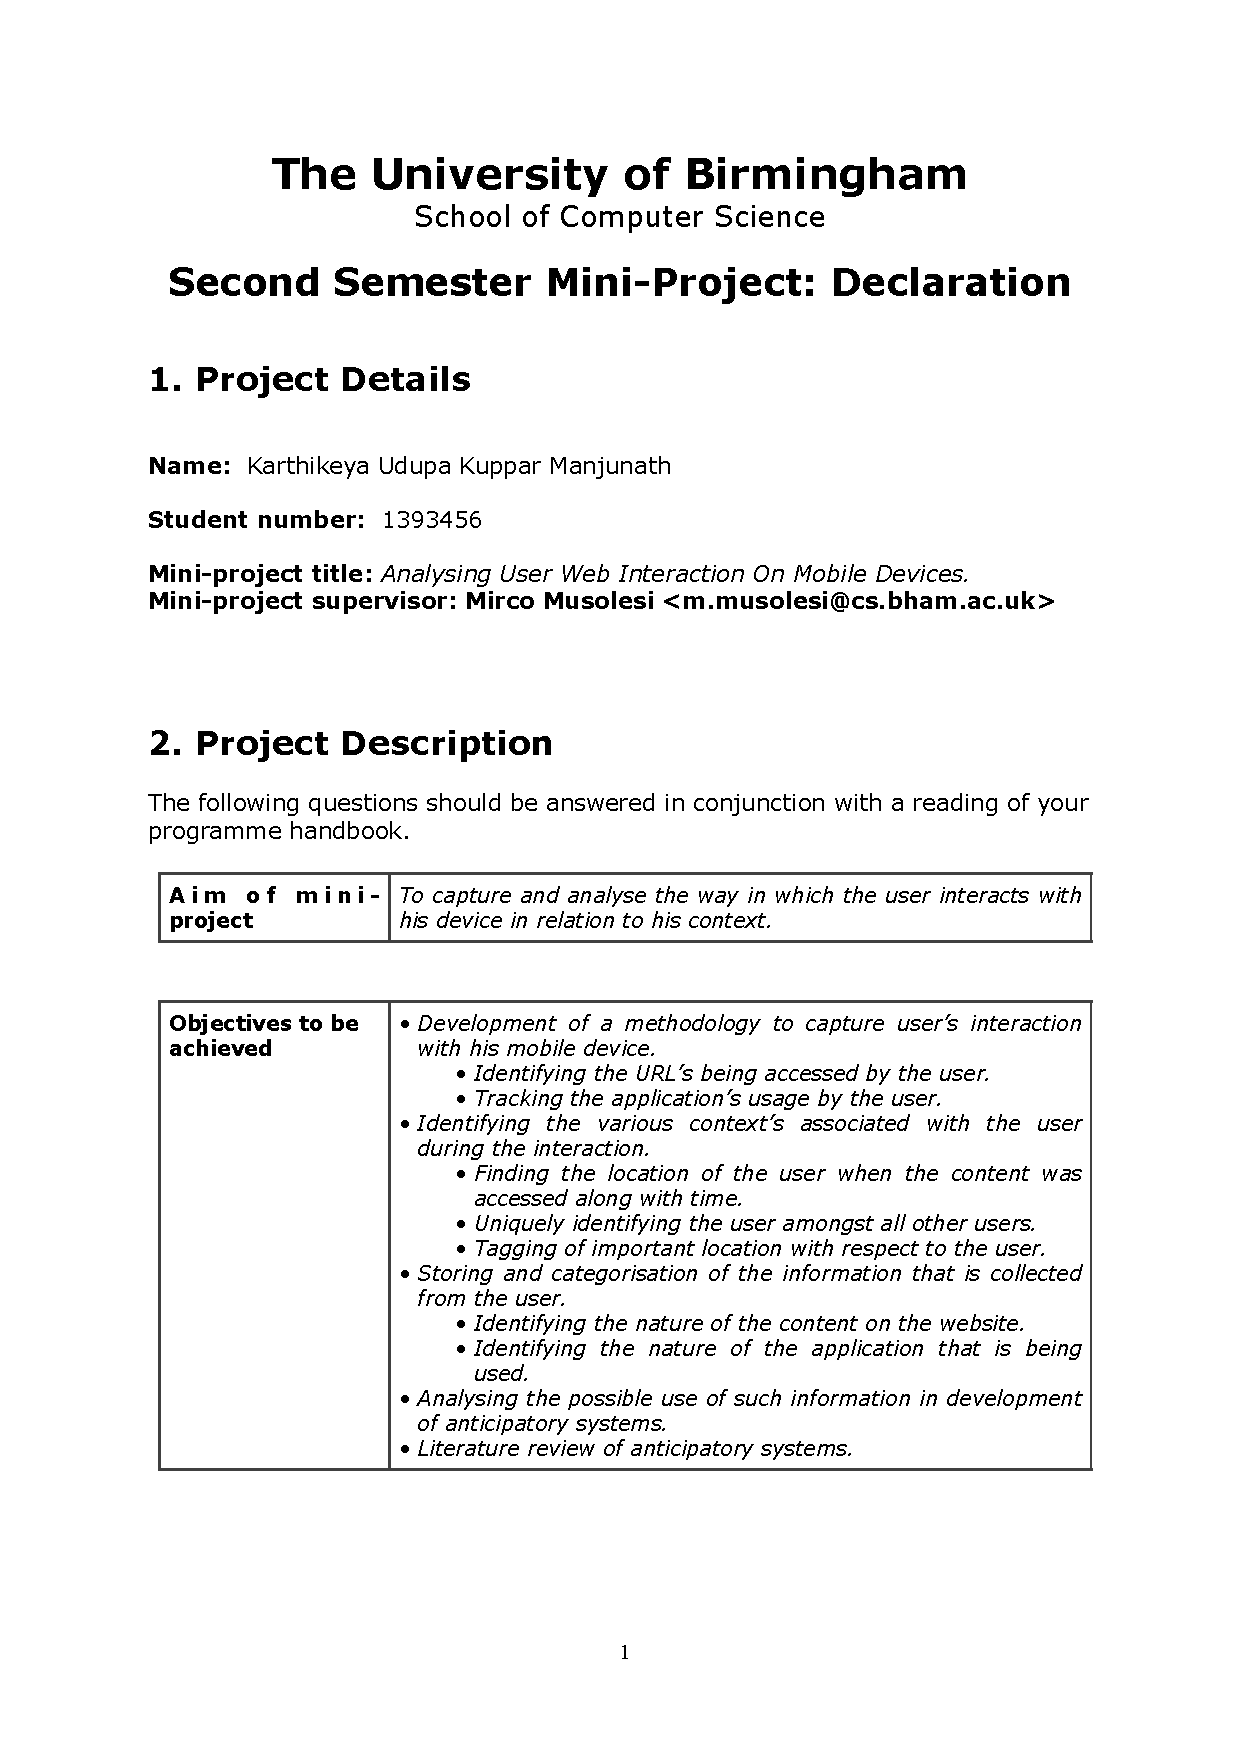
\includepdf[pages={1,2}]{Declaration.pdf}

\chapter{Statement of information search strategy}

statement of search
\end{document}